\documentclass{article}
\usepackage[spanish]{babel}
\usepackage{float}
\usepackage{amsmath}
\usepackage{amssymb}
\usepackage{multicol}
\usepackage[colorlinks=true, linkcolor=black, citecolor=black, urlcolor=black]{hyperref}
\usepackage{graphicx} % Para incluir imágenes
\usepackage{enumitem} % Para personalizar listas

\begin{document}

\tableofcontents
\newpage


\section{¿Qué es la estadística?}
    La estadística es una \textbf{herramienta fundamental} para realizar una investigación científica. Su finalidad es conocer el problema, obtener conclusiones y tomar decisiones. Ofrece un conjunto de métodos y técnicas para:

    \begin{multicols}{2}
    \begin{itemize}
    \item Recolectar
    \item Clasificar
    \item Procesar
    \item Presentar
    \item Analizar
    \item Interpretar
    \end{itemize}
    \end{multicols}

    \subsection{División de la Estadística}

        \subsubsection{Estadística Descriptiva}
            Describe y resume los datos observados mediante gráficos o cuadros, mostrando indicadores de cálculo (media, mediana, moda, etc.).

        \subsubsection{Estadística Inferencial}
            Permite generalizar acerca de una población a partir de lo observado en una muestra.

    \subsection{Definiciones}

        \subsubsection{Población}
            Conjunto de todas las \textbf{unidades de estudio} que cumplen ciertas características de interés. Se clasifican en \text{Extensión} y \text{Naturaleza}
            

        \subsubsection{Unidad de Estudio}
            Es el objeto o elemento indivisible que brindará la información de lo estudiado.

        \subsubsection{Muestra}
            Subconjunto de la población en estudio. Sus características principales son \textbf{representativa} y \textbf{adecuada}.

        \subsubsection{Variable}
            Característica de la población que se va a estudiar, y puede tomar diferentes valores (edad, género, estado civil, talla, etc.).

            \paragraph{Clasificación de las Variables}
            \begin{itemize}[label=-]
            \item \textbf{Variable Cualitativa}
            \begin{itemize}
            \item \textbf{Nominal}: Categorías sin orden preestablecido (género, estado civil).
            \item \textbf{Ordinal}: Categorías con un orden preestablecido (grado de instrucción).
            \end{itemize}

            \item \textbf{Variable Cuantitativa}
            \begin{itemize}
            \item \textbf{Discreta}: Toma valores enteros (número de artículos vendidos).
            \item \textbf{Continua}: Toma cualquier valor dentro de un intervalo (edad, talla).
            \end{itemize}
            \end{itemize}

        \subsubsection{Parámetro}
            Medida resumen que describe una característica de la población.
            Parámetros más usados:
            \begin{itemize}
            \item La media poblacional: $\mu$
            \item La proporción poblacional: $P$
            \item La desviación estándar poblacional: $\sigma$
            \end{itemize}

        \subsubsection{Estadístico o Estadígrafo}
            Medida que describe una característica de la muestra.
            Parámetros más usados:
            \begin{itemize}
            \item La media muestral: $\bar{x}$
            \item La proporción muestral: $\hat{p}$
            \item La desviación estándar muestral: $S$
            \end{itemize}
            

\section{Recolección de datos}
    Implica elaborar un plan detallado de procedimientos para reunir datos con un propósito específico. Esto nos permite determinar:

    \begin{itemize}
    \item ¿Cuáles son las fuentes de donde vamos a obtener los datos?
    \item ¿Dónde se localizan esas fuentes?
    \item ¿A través de qué método vamos a recolectar los datos?
    \item ¿De qué forma vamos a preparar los datos recolectados para su análisis?
    \end{itemize}

    \subsection{Técnicas de recolección de datos}
        Comprenden procedimientos que permiten obtener la información necesaria a la pregunta de investigación.
        
        \begin{multicols}{2}
        \begin{enumerate}[label=\arabic*.]
        \item Encuesta
        \item Entrevista
        \item Observación
        \item Análisis Documental
        \end{enumerate}
        \end{multicols}

    \subsection{Instrumentos de Recolección}
    Son las vías mediante las cuales es posible aplicar una técnica de recolección de información.

        \begin{table}[h!]
            \centering
            \begin{tabular}{|c|c|}
                \hline
                \multicolumn{2}{|c|}{\textbf{Técnicas directas}} \\\hline
                \textbf{Técnicas} & \textbf{Instrumentos} \\\hline
                Observación & Ficha de Observación \\\hline
                \multicolumn{2}{|c|}{\textbf{Técnicas indirectas}} \\\hline
                \textbf{Técnicas} & \textbf{Instrumentos} \\\hline
                Encuesta & Cuestionario de Encuesta \\\hline
                Entrevista & Cuestionario de Entrevista \\\hline
                Análisis Documental & Ficha de análisis documental \\\hline
            \end{tabular}
            \caption{Instrumentos de recolección}
        \end{table}

    \subsection{Pasos para elaborar un Cuestionario de Encuesta}
        \begin{enumerate}[label=\arabic*.]
        \item Determinar el objetivo del cuestionario.
        \item Determinar las variables que intervienen.
        \item Determinar los indicadores de cada variable.
        \item Mediante una lluvia de ideas, determinar preguntas para cada indicador.
        \item Análisis de las preguntas para cada indicador.
        \item Elaborar el primer proyecto de cuestionario.
        \item Elaborar la matriz de consistencia.
        \item Realizar una prueba piloto.
        \item Corregir el cuestionario y elaborar un nuevo proyecto.
        \item Obtener el cuestionario definitivo.
        \end{enumerate}

        \subsubsection{Partes del Cuestionario}
            \begin{multicols}{2}
                \begin{enumerate}[label=\arabic*.]
                \item Encabezado
                \item Flujo del Cuestionario
                \item Preguntas de calentamiento
                \item Preguntas de transición
                \item Cierre
                \end{enumerate}
            \end{multicols}

        \subsubsection{Tipos de Preguntas}
            \begin{enumerate}[label=\arabic*.]
                \item Preguntas de respuestas abiertas
                    \begin{itemize}
                    \item \textbf{Básica:} ¿Qué le gustó más de ese producto?
                    \item \textbf{De Seguimiento:} ¿Qué más le gustó del producto?
                    \end{itemize}

                \item Preguntas de respuestas cerradas (dicotómicas)
                    \begin{itemize}
                        \item ¿Ha comido usted alguna vez carne de cordero?
                        \begin{multicols}{2}
                        \begin{enumerate}[label=\alph*.]
                        \item Sí
                        \item No
                        \end{enumerate}
                    \end{multicols}
                    \end{itemize}

                \item Preguntas de respuestas múltiples
                    \begin{itemize}
                        \item ¿Cuáles de los siguientes productos incluyó la última vez que fue a un supermercado?
                            \begin{enumerate}[label=\alph*.]
                            \item Alimentos y bebidas no alcohólicas
                            \item Productos de aseo del hogar
                            \item Productos de aseo personal
                            \item Bebidas alcohólicas
                            \item Productos farmacéuticos
                            \end{enumerate}
                    \end{itemize}

                \item Preguntas de respuestas cerradas a escala
                    \begin{itemize}
                        \item ¿Te interesa la carrera Computación Científica?
                            \begin{multicols}{2}
                            \begin{itemize}
                            \item Extremadamente interesante
                            \item Muy interesante
                            \item Bastante interesante
                            \item Algo interesante
                            \item Poco interesante
                            \item Nada interesante
                            \end{itemize}
                            \end{multicols}
                    \end{itemize}
            \end{enumerate}

\section{Gráficos de Organización de Datos}
    \subsection{Organización de los Datos}
        Es necesario resumir la información recolectada y presentar los datos de manera que faciliten su comprensión y posterior análisis.

    \subsection{Tabla o Distribución de Frecuencias}
        \begin{itemize}
            \item Representación de una serie de datos que muestra cómo se distribuye una variable estadística junto con sus frecuencias.
            \item Arreglo ordenado en columnas y filas de datos numéricos y características relacionadas, facilitando la lectura, comparación e interpretación.
        \end{itemize}

        \subsubsection{Partes de una Tabla de Frecuencias}
            \begin{enumerate}[label=\arabic*.]
                \item Número del cuadro de frecuencias en forma correlativa.
                \item Título: Especificar la variable y la población en estudio.
                \item Encabezado o Conceptos.
                \item Cuerpo o contenido del cuadro de frecuencias.
                \item Nota de pie.
                \item Fuente.
                \item Elaboración.
            \end{enumerate}

            \begin{figure}[h!]
                \centering
                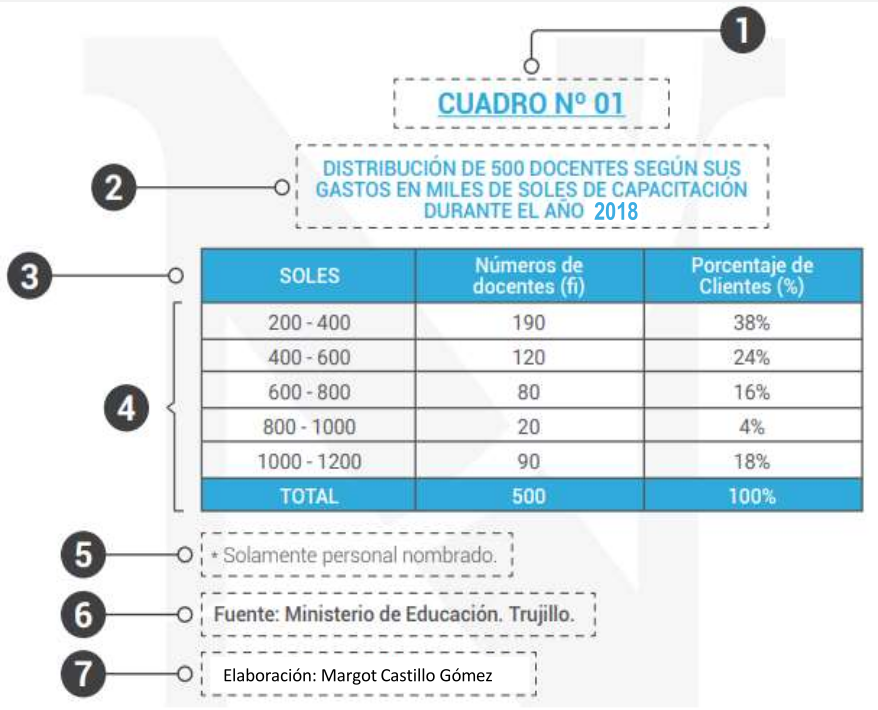
\includegraphics[width=0.8\textwidth]{img/tabla_frecuencia.png}
                \caption{Ejemplo de tabla de frecuencias}
            \end{figure}

    \subsection{Distribución de Frecuencias}
        \subsubsection{Variables Cualitativas}
            \begin{table}[H]
                \centering
                \begin{tabular}{|c|c|c|c|}
                    \hline
                    & \textbf{Frecuencias} & \textbf{Frecuencias} &  \\
                    \textbf{Categoría} & \textbf{Absolutas } & \textbf{ Relativas } & \textbf{Porcentajes } \\
                    & \textbf{($f_i$)} & \textbf{ ($h_i$)} & \textbf{($p_i = h_i \cdot 100\%$)} \\ \hline
                    $C_1$& $f_1$  & $h_1$ & $p_1$ \\ 
                    $C_2$& $f_2$  & $h_2$ & $p_2$ \\ 
                    $\vdots$& $\vdots$  & $\vdots$ & $\vdots$ \\ \hline
                    \text{Total} & n & 1 & $100\%$ \\ \hline
                    &&&\\
                    Ordenar ascendente & \#N de datos & $h_i = \cfrac{f_i}{n}$ & $h_i = \cfrac{f_i}{n}\cdot 100\%$ \\ 
                    &&&\\ \hline
                \end{tabular}
                \caption{Distribución de Frecuencias Cualitativas}
            \end{table}

            \textbf{Gráficos para Variables Cualitativas}
                \begin{itemize}
                    \item\textbf{Diagrama de sectores} (tartas, polares): 
                    \item\textbf{Diagrama de Barras}: Alturas 
                \end{itemize}
            

        \subsubsection{Variables Cuantitativa Discreta}
            \begin{table}[H]
                \centering
                \begin{tabular}{|c|c|c|c|c|}
                    \hline
                    & \textbf{Frecuencias}& \textbf{Frecuencias}&\textbf{Frecuencias} &\textbf{Frecuencias}  \\
                    \textbf{Variable}   & \textbf{Absolutas } & \textbf{acumulada}&\textbf{ Relativas } & \textbf{Acumulada} \\
                    $x_i$ & \textbf{($f_i$)}    & $F_i$&\textbf{ ($h_i$)}    & \textbf{($H_i$)} \\ \hline
                    $C_1$& $f_1$  & $F_1$ & $h_1$ & $H_1$\\ 
                    $C_2$& $f_2$  & $F_2$ & $h_2$ & $H_2$\\ 
                    $\vdots$& $\vdots$  & $\vdots$ & $\vdots$ & $\vdots$ \\ 
                    $\vdots$& $\vdots$  & n & $\vdots$ & 1\\\hline
                    \text{Total} & n & &1 & \\ \hline
                    &&&&\\
                    & \#n de datos & &$h_i = \cfrac{f_i}{n}$ &  \\ 
                    &&&&\\ \hline
                \end{tabular}
                \caption{Distribución de Frecuencias Cuantitativa Discreta}
            \end{table}

            \textbf{Gráficos para Variables Cuantitativa Discreta}
            \begin{itemize}
                \item\textbf{Grafico de Bastón} 
            \end{itemize}

            
        
        \subsubsection{Variables Cuantitativa Continua}
            \subsubsection*{Pasos a Seguir:}
                \begin{table}[H]
                    \begin{tabular}{|c|c|}
                        \hline
                        \textbf{Determinar El rango} & $R = V_{max} - V_{min}$ \\ \hline
                        \textbf{Determinar el n° de intervalor} & $m = 1 + 3.32\log{n}$ \\ \hline
                        \textbf{Determinar la amplitud de cada intervalo}  & $C = \cfrac{R}{m}$ \\ \hline
                        \textbf{Establecer los intervalos de clase} &\\\hline
                    \end{tabular}
                \end{table}
                \begin{figure}[H]
                    \centering
                    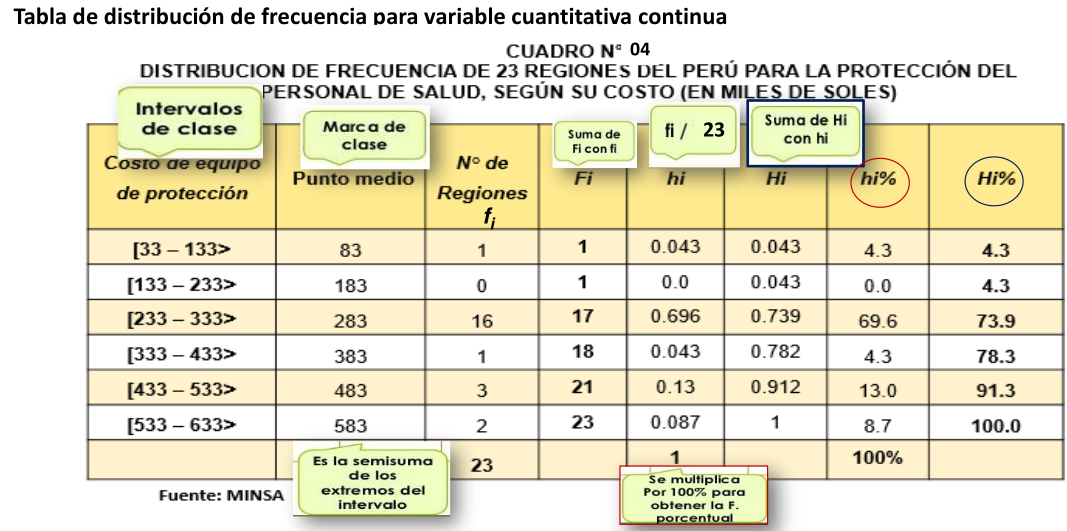
\includegraphics[width=0.9\textwidth]{img/tabla_2.png}
                    \caption{Tabla de frecuencia variable cuantitativa continua}
                \end{figure}
                \begin{table}[H]
                    \centering
                    \begin{tabular}{|c|c|}
                        \hline
                        Rango & $R = V_{max} - V_{min} = 632 - 33 = 599$ \\ \hline
                        n° de intervalos & $m = 1 + 3.32\log{23}= 2.52=6$ \\ \hline
                        Amplitud de cada intervalo  & $C = \cfrac{599}{6}= 99.83=100$ \\ \hline
                    \end{tabular}
                \end{table}
            \subsubsection*{Gráficos para Variables Cuantitativa Continua}
                \begin{itemize}
                    \item\textbf{Histograma de Frecuencias} 
                    \item \textbf{Poligono de Frecuencias} 
                \end{itemize}

\section{Medidas de Tendencia Central}    
    Son valores representativos de la totalidad de los datos. Su cálculo permite analizar los datos en torno a un valor central.
    Los más usados son: Media Artimetica, Mediana y Moda.
    \subsection{Media Aritmética (\texorpdfstring{$\bar{x}$}{x-bar})}
        \begin{itemize}
            \item Es sensible a la variación de las puntuaciones.
            \item No es \textbf{recomendable} cuando hay \textbf{valores muy extremos}.
        \end{itemize}
        \subsubsection{Fórmulas de Media}
            \begin{table}[H]
                \centering
                \begin{tabular}{|c|c|c|}
                    \hline
                    &Datos sin agrupar&Datos agrupados \\ \hline
                    Población& $\mu = \sum_{i=1}^{n}\cfrac{x_i}{N}$&$\mu = \sum_{i=1}^{n}\cfrac{x_i\cdot f_i}{N}$ \\ \hline
                    Muestra & $\bar{x} = \sum_{i=1}^{n}\cfrac{x_i}{n}$ & $\bar{x} = \sum_{i=1}^{n}\cfrac{x_i\cdot f_i}{n}$ \\ \hline
                \end{tabular}
            \end{table}
        \subsubsection{Ejemplos}
            \begin{figure}[h!]
                \centering
                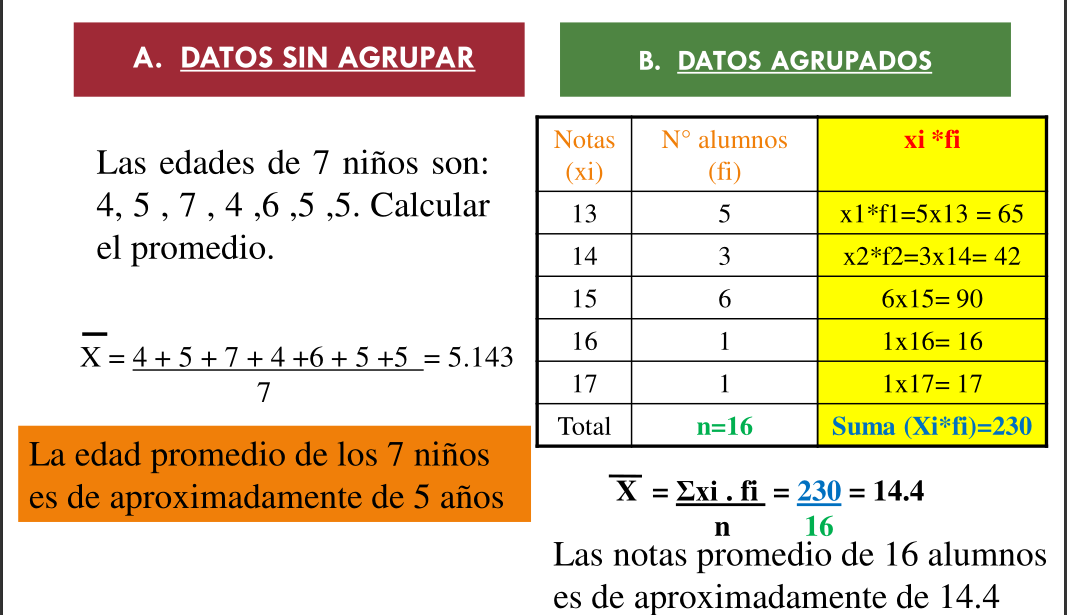
\includegraphics[width=0.8\textwidth]{img/media1.png}
                \caption{Ejemplo de Media}
            \end{figure}
            \begin{figure}[h!]
                \centering
                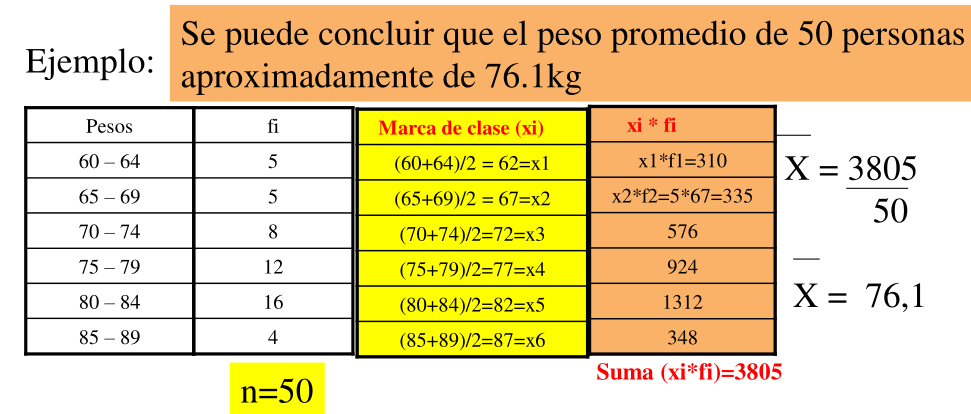
\includegraphics[width=0.8\textwidth]{img/media2.png}
                \caption{Ejemplo para datos agrupados con intervalos}
            \end{figure}
    \subsection{Mediana (Me)}
        Valor de la variable que divide a los datos en dos partes iguales o deja igual número de valores antes y después de él en una distribución de frecuencias.
        \textbf{NOTA: Para obtener la media, los valores deben estar ordenados. Puede ser en forma creciente o decreciente.}
        \subsubsection{Fórmulas con datos sin Agrupar}
        \begin{table}[H]
            \centering
            \begin{tabular}{|c|c|c|}
                \hline
                n impar& $ i = \cfrac{n+1}{2}$&$ Me = x_i$ \\ &&\\ \hline 
                n par  & $i = \cfrac{n}{2}$&$ Me = \cfrac{x_i + x_{i+1}}{2}$ \\ &&\\ 
                \hline
            \end{tabular}
        \end{table}
        \subsubsection{Fórmulas con datos Agrupados}
            \[Me = L_i + A\cdot\left[\cfrac{\frac{n}{2} - F_{i-1}}{F_i - F_{i-1}}\right]\]
            \begin{itemize}
                \item $n$: Numero total de datos
                \item $L_i$: Limite inferior del intervalo critico seleccionado
                \item $F_i$: Frecuencia acumulada del intervalo seleccionado ($F_i \geq \frac{n}{2}$)
                \item $F_{i-1}$: Frecuencia acumulada del intervalo anterior
                \item $A$: Amplitud del intervalo                
            \end{itemize}

        \subsubsection{Ejemplos}
            \begin{figure}[H]
                \centering
                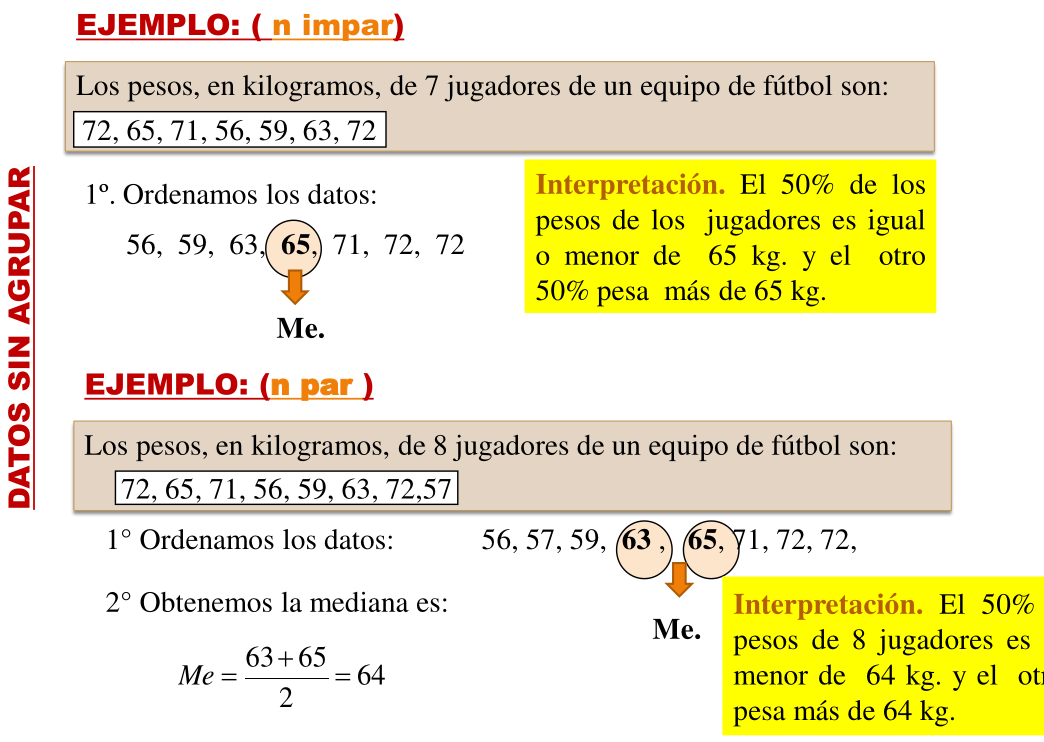
\includegraphics[width=0.8\textwidth]{img/mediana1.png}
                \caption{Datos no agrupados}
                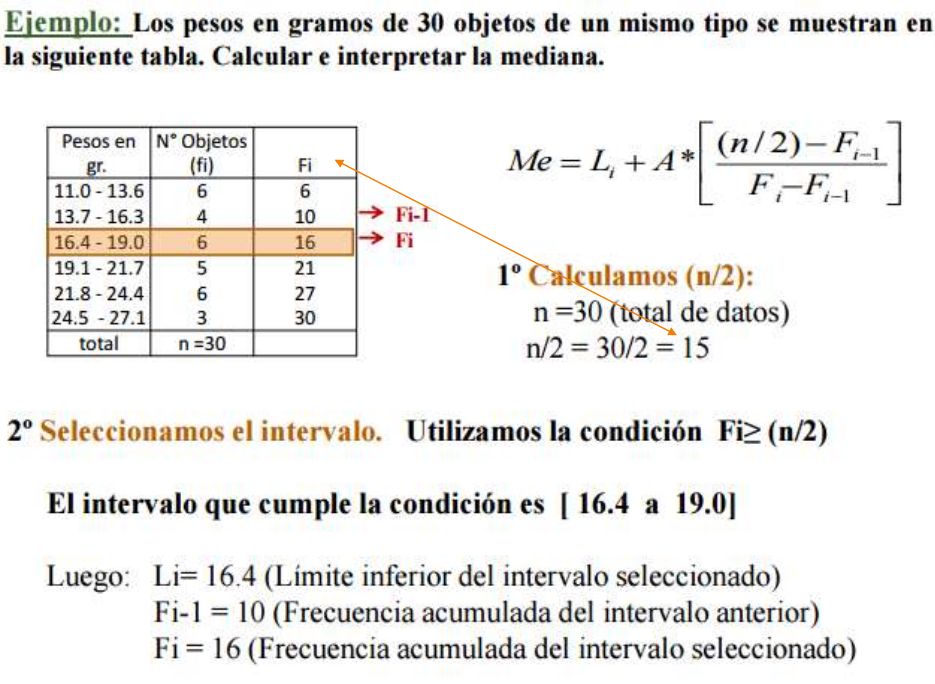
\includegraphics[width=0.8\textwidth]{img/mediana2.png}
                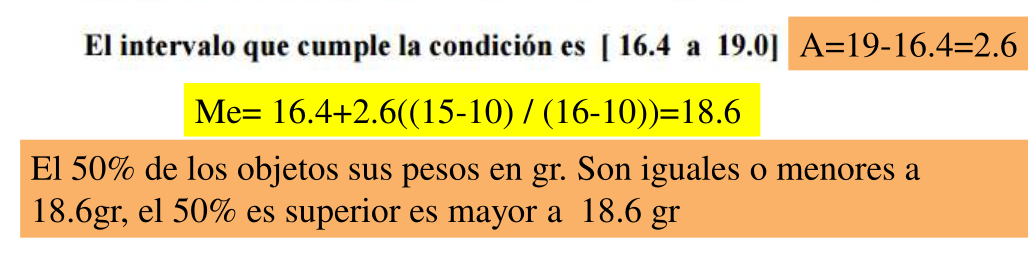
\includegraphics[width=0.8\textwidth]{img/mediana3.png}
                \caption{Datos agrupados}
            \end{figure}
    
    \subsection{Moda (Mo)}
        Es el valor o característica de la variable que más se repite o que tiene mayor frecuencia. Se utiliza en variables \textbf{cualitativas} y \textbf{cuantitativas}.
        
        \subsubsection{Ejemplos}
            \begin{figure}[H]
                \centering
                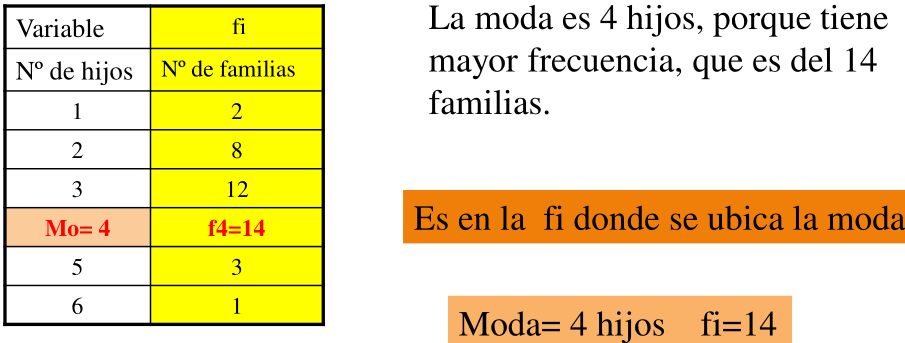
\includegraphics[width=0.8\textwidth]{img/moda1.png}
                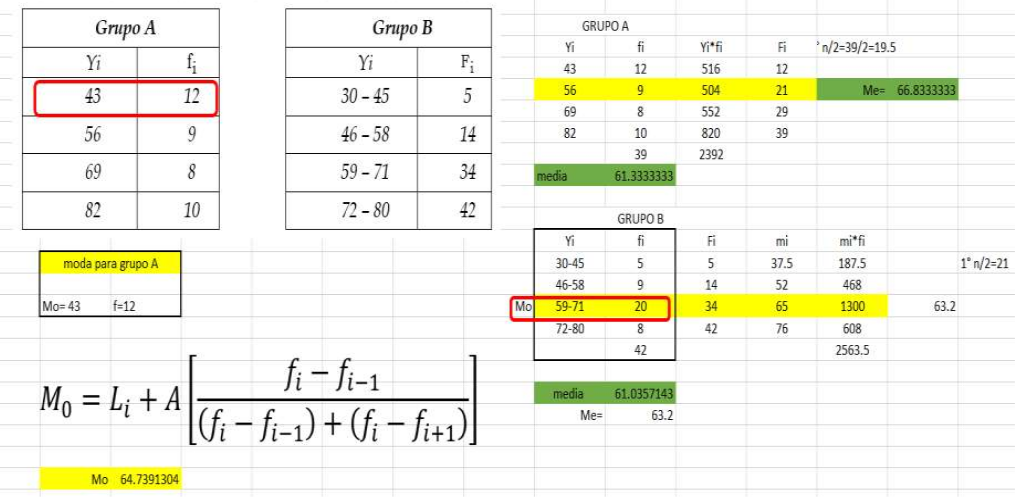
\includegraphics[width=0.8\textwidth]{img/moda2.png}
            \end{figure}

\section{Medidas de Dispersión}
    \begin{itemize}
        \item Los datos se dispersan alrededor de su punto central (media).
        \item La variabilidad mide la distancia promedio de los datos a su valor central.
        \item Una mayor variabilidad indica que los datos están más alejados de la media.
        \item Una menor variabilidad sugiere que los datos son más homogéneos en relación a la media.
    \end{itemize} 
    \subsection{Absolutas}
        \subsubsection{Recorrido (Rango)}
            Se determina restando el valor maximo y minimo, de los datos. $R = V_{max} - V_{min}$
        \subsubsection{Varianza }
            Mide la mayor o menor dispersión de los valores de la variable respecto a la media ritmetica. Se expresa en las mismas unidades que la variable analizada, pero elevadas al cuadrado
            \begin{multicols}{2}
                \begin{itemize}
                    \item $X_i$: Valores de la variable x
                    \item $Y_i$: marca de clase de cada variable
                    \item $N$: Tamaño de la población
                    \item $n$: Tamaño de la muestra
                    \item $\sigma^2$: Varianza poblacional
                    \item $S^2$: Varianza muestral
                \end{itemize}
            \end{multicols}
            \begin{table}[H]
                \centering
                \begin{tabular}{|c|c|c|c|}
                    \hline
                    & Datos sin agrupar & Datos agrupados & Abreviada \\ \hline &&&\\
                    Población & $\sigma^2 = \cfrac{\sum_{i=1}^{N}(x_i - \mu)^2}{N}$ &$\sigma^2 = \cfrac{\sum_{i=1}^{N}(Y_i - \mu)^2\cdot f_i}{N}$ & $\sigma^2= \cfrac{\sum_{i=1}^{N}X_i^2f_i}{N} - \mu^2$ \\ &&&\\ \hline &&&\\
                    Muestra & $S^2 = \cfrac{\sum_{i=1}^{n}(x_i - \bar{x})^2}{n-1}$ & $S^2 = \cfrac{\sum_{i=1}^{n}(Y_i - \bar{x})^2\cdot f_i}{n-1}$ & \\ &&&\\\hline
                \end{tabular}
            \end{table}
        \subsubsection{Desviación Estandar}
            Conocidad también como la \textbf{desviación típica} y es la medida que nos indica cuánto tiende a alejarse los datos del promedio. Se calcula sacando la raíz cuadrada de la varianza.
            \begin{table}[H]
                \centering
                \begin{tabular}{|c|c|}
                    \hline
                    Población & $\sigma = \sqrt{\sigma^2}$ \\ \hline
                    Muestra & $S = \sqrt{S^2}$ \\ \hline
                \end{tabular}
            \end{table}
    \subsection{Relativas}
        \subsubsection{Coeficiente de Variancia}
        Permite comparar la variabilidad de dos o más conjuntos de datos expresados en unidades diferentes.
        \[CV = \cfrac{S}{\bar{x}}\cdot 100\]
        \subsubsection{Ejemplos}
        \begin{figure}[H]
            \centering
            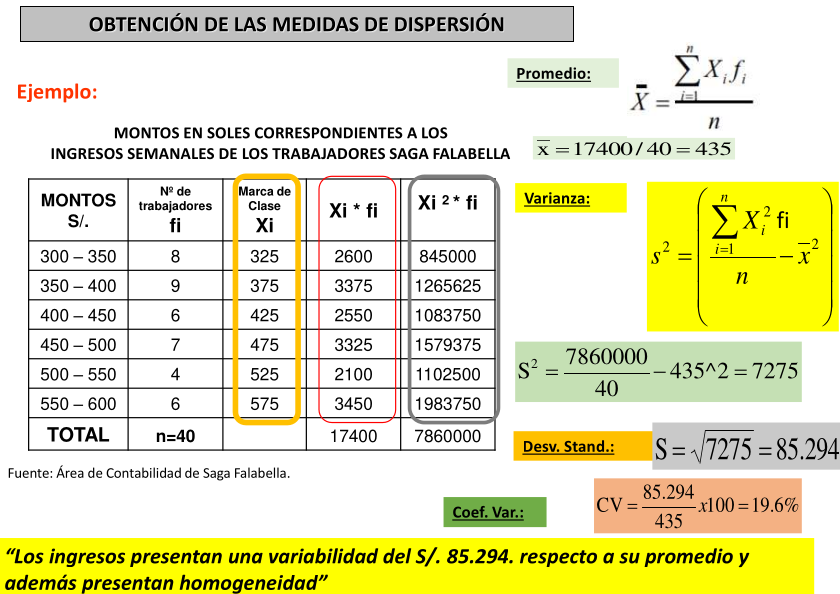
\includegraphics[width=0.8\textwidth]{img/dispersion.png}
        \end{figure}
\section{Medidas de Tendencia No Central}
    Nos permiten conocer otras medidas características del conjunto de datos que no son los valores centrales, estas medidas se conocen con el nombre de cuantiles
    \begin{enumerate}
        \item\textbf{Percentil}: Dividen al conjunto de datos en cien partes iguales
        \item\textbf{Decil}: Dividen al conjunto de datos en diez partes iguales
        \item\textbf{Cuartiles}: Dividen al conjunto de datos en cuatro partes iguales
    \end{enumerate}
    \begin{figure}[H]
        \centering
        \begin{minipage}{0.5\textwidth}
            \centering
            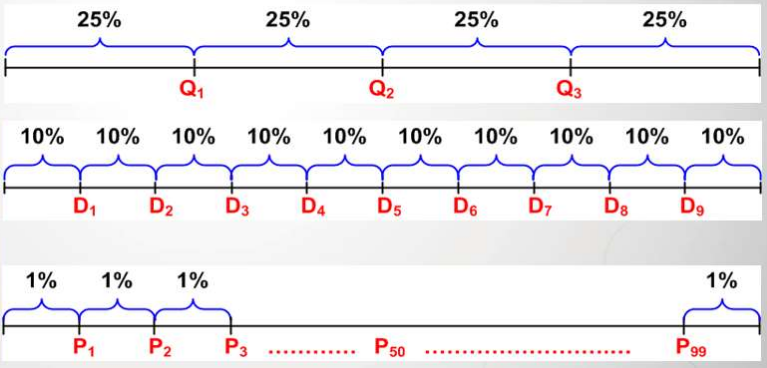
\includegraphics[width=\textwidth]{img/noCentral.png}
        \end{minipage}%
        \hfill
        \begin{minipage}{0.5\textwidth}
            \centering
            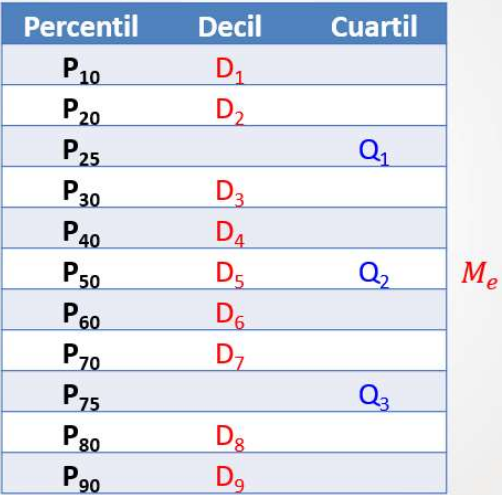
\includegraphics[width=\textwidth]{img/equivalencia.png}
        \end{minipage}
    \end{figure}
    
    \subsection{Percentil con datos no agrupados}
        \begin{enumerate}
            \item Ordenarlos datos en forma ascendente
            \item Hallar la posicion ($j$) del percentil $P_k$ a partir de las siguientes expresión: \[j=\cfrac{k\cdot(n+1)}{100}\]
            \item Ubicar el percentil en la posicion hallada si "j" es un número entero; caso contrario, el percentil se calcula con las siguiente fórmula: \[P_k = L_i + dec\cdot (L_d-L_i)\]
            \[L_i:\text{Limite izquierdo}\quad L_d:\text{Limite derecho}\quad dec:\text{Parte decimal de la posicion}\] 
        \end{enumerate}
        \begin{figure}[H]
            \centering
            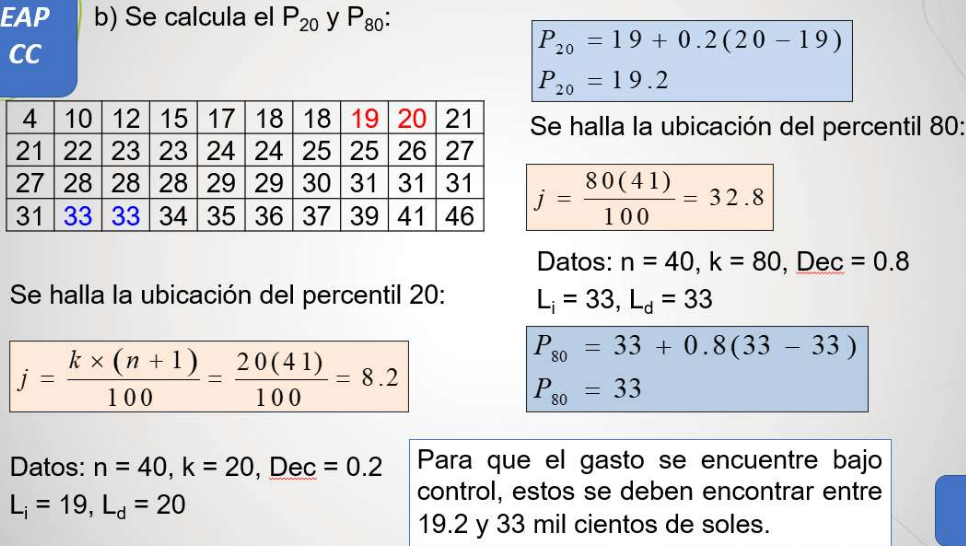
\includegraphics[width=0.8\textwidth]{img/percentil.png}
        \end{figure}
    
    \subsection{Diagrama de Caja}
        Representacion gráfica de la distribucion de un variable cuantitativa. Esta compuesta por un rectangulo  y dos lineas extendidas, acada lado llamadas bigotes.
        Para construir un diagrama de caja se procede de la siguiente manera:
        \begin{itemize}
            \item Ordenar los datos de menor a mayor
            \item Calcular los cuatiles: $Q_1$, $Q_2$(Me) y $Q_3$
            \item Calcular el rango de intercuartilico: $R_i = Q_3 - Q_1$
            \item Calcular $a = Q_1 - 1.5\cdot R_i$ y $b = Q_3 + 1.5\cdot R_i$
                \begin{itemize}
                    \item Los datos fuera del intervalo $[a,b]$ son considerados datos atípicos (outliers); es posible que en una distribucion no se encuentren este tipo de datos. En el grafico de cajas, los datos atípicos son represntados mediante asteriscos.
                \end{itemize}
            \item Ubicar el dato con menor valor y el dato con mayor valor en el intervalo $[a,b]$
        \end{itemize}
        \subsubsection{Medidas de Forma}
        o.
        \begin{enumerate}
            \item\textbf{Coefiente de Asimetria}
                Estas medidas brindan información sobre la dirección horizontal que toma la distribución de los datos con respecto a su centro.
                \[A_k = \cfrac{3(\bar{X} - Me)}{S}\]
                \begin{itemize}
                    \item $A_k<0$: la distribucion es asimetrica negativa o hacia la izquierda
                    \item $A_k=0$: la distribucion es simetrica
                    \item $A_k>0$: la distribucion es asimetrica positiva o hacia la derecha
                \end{itemize}
                \begin{figure}[H]
                    \centering
                    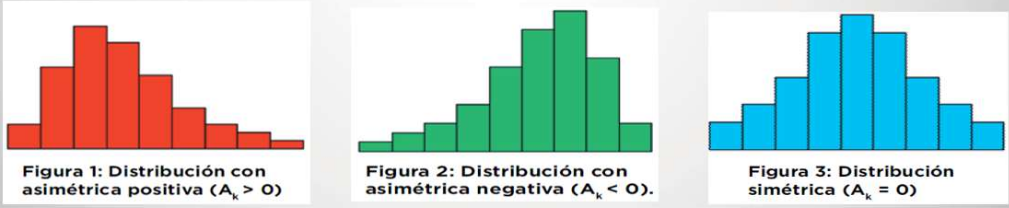
\includegraphics[width=0.8\textwidth]{img/asimetria.png}
                \end{figure}
            \item\textbf{Coefiente de Cutorsis}
                Esta medida brinda informacion sobre la deformacion vertical de una distribucion de frecuencias en comparacion con la curva normal
                \[K_u = \cfrac{Q_3 - Q_1}{2(P_{90} - P_{10})} = \cfrac{P_{75} - P_{25}}{2(P_{90} - P_{10})}\]
                \begin{itemize}
                    \item $K_u<0.263$: la distribucion es Platicúrtica
                    \item $K_u=0.263$: la distribucion es Mesocútica
                    \item $K_u>0.263$: la distribucion es Leptocúrtica
                \end{itemize}
                \begin{figure}[H]
                    \centering
                    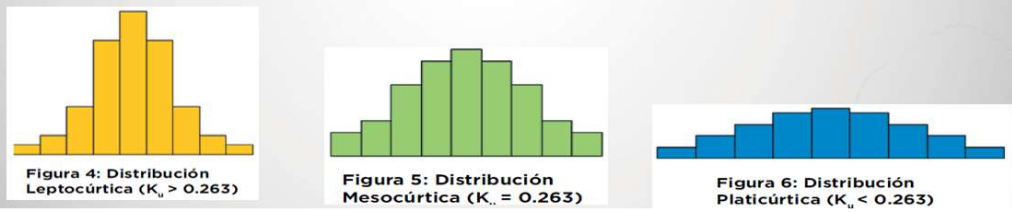
\includegraphics[width=0.8\textwidth]{img/kutorisis.png}
                \end{figure}
        \end{enumerate}
    \subsection{Diagrama Tallo y Hoja}
        Permite obtener simultáneamente uns distribucion de frecuencias, que es la representacion estructrada en forma de tabla. El \textbf{tallo} es usado para agrupar los valores y cada \textbf{hoja} indica los valores individuales dentro de cada grupo.
        \subsubsection{Constrcción del diagrama}
            \begin{itemize}
                \item Ordenar los datos de forma ascendente.
                \item Construir las columnas de tallo y la hoja
                \item Completa la columna de tallo con las decenas y las hojas con las unidades
                \item Completamos la frecuencia con la cantidad de hojas que tiene cada tallo.
            \end{itemize}
            \begin{figure}[H]
                \centering
                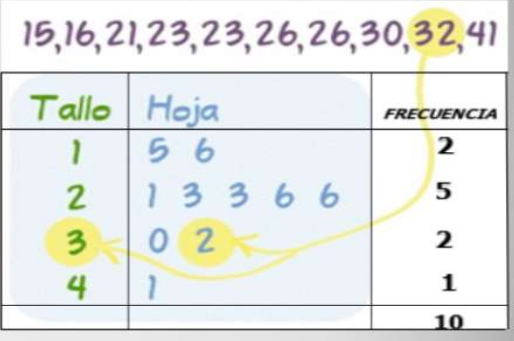
\includegraphics[width=0.6\textwidth]{img/tallo.png}
            \end{figure}

\section{Probabilidades}
    \subsection{Conceptos}
        \subsubsection{\texorpdfstring{Experimento ($\xi$)}{Experimento (xi)}}
            Es cualquier acción o procesos que genera observaciones lo cual puede ser:
            \begin{enumerate}
                \item\textbf{Deterministico}: Experimento que al repetirse bajo las mismas condiciones este genera los mismo resultados
                \item \textbf{Aleatorio}: Experimento que bajo las mismas condiciones no genera siempre los mismo resultados.
            \end{enumerate}
        \subsubsection{\texorpdfstring{Espacio Muestral ($\Omega$)}{Espacio Muestral (Omega)}}
            Se llama espacio muestral de $\xi$, de notado por $\Omega$, al conjunto de todos los resultados posibles del expermiento.
            \[\xi:\quad\Omega =\{\omega_1, \omega_2, \dotsc,\omega_n\}\]
        \subsubsection{Suceso o Evento (A, B, C, ...)}
            Es cualquier subconjunto del espacio muestral $\Omega$. Contiene resultados de un expermiento aleatorio que tienen una caracteristica particular. 
            \subsubsection{Operaciones con Eventos}
                \begin{enumerate}
                    \item\textbf{Union}: $A\cup B = \{w\in\Omega | w\in A \land w\in B\}$
                    \item\textbf{Intersección}: $A\cap B = \{w\in\Omega | w\in A \lor w\in B\}$
                        \begin{itemize}
                            \item\textbf{$A\cap B = \emptyset$, se dice que los eventos son excluenyes o disjuntos}
                        \end{itemize}
                    \item\textbf{Complemento}: $\bar{A}=\{w\in\Omega | w\notin A\}$
                \end{enumerate}
    
    
    
    \subsection{Enfoques de la Probabilidad}
        \subsubsection{Probabilidad Clásica}
            \[P(E) = \cfrac{\#\text{Casos a favor de E}}{\#\text{Casos posibles}} = \cfrac{n(E)}{n(\Omega)}\]
        
        \subsubsection*{Teoremas de Probabilidades}
        \begin{enumerate}
            \item $0\leq P(E) \leq 1$
            \item $P(\emptyset) = 0 \quad\land\quad P(\Omega)=1$
            \item $P(\bar{E})=1-P(E)$
            \item $P(E-F)= P(E)-P(E\cap F)$
            \item $P(E\cup F) = P(E)+P(F)\quad si:\quad E\cap F = \emptyset$
            \item $P(E\cup F) = P(E)+P(F) - P(E\cap F)\quad si:\quad E\cap F \neq \emptyset$
            \item $P(E)\leq P(F)\quad Si:\quad E\subseteq F$
        \end{enumerate}
        \subsubsection*{Probabilidad Condicional}
            \[P(B|A) =\cfrac{P(B\cap A)}{P(A)}\]
            Si son dos eventos independientes tenemos:
            \[P(A|B) = P(A)\quad\land\quad P(A\cap B) = P(A)\cdot P(B)\]
    
    \subsection{Principo de Multiplicación}
        Este principio es útil si es de interés calcular la probabilidad de que ocurran los n eventos de manera simultánea.
        \begin{itemize}
            \item Para dos eventos  \[P(A\cap B)= P(A)P(B|A)\]
            \item Para n eventos \[P(\bigcap_{i=1}^{n}A_i) = P(A_1)\prod_{i=2}^{n}P(A_i| \bigcap_{j=1}^{i-1}A_j)\]
        \end{itemize}
    
    \subsection{Teorema de Porbabilidad Total}
        Sean \( A_1, A_2, \ldots, A_n \) una colección de eventos mutuamente excluyentes con probabilidades conocidas y cuya unión es el espacio muestral, es decir:
        \[\Omega = A_1 \cup A_2 \cup \cdots \cup A_n.\]
        Sea \( A \) un evento cualquiera que satisface:
        \[A = (A \cap A_1) \cup (A \cap A_2) \cup \cdots \cup (A \cap A_n)\]
        con probabilidades condicionales conocidas \( P(A | A_i) \); \( i = 1, 2, \ldots, n \). Entonces, la probabilidad del evento \( A \) se calcula de la siguiente manera:
        \[P(A) = P(A_1) \times P(A | A_1) + P(A_2) \times P(A | A_2) + \cdots + P(A_n) \times P(A | A_n).\]
        Esta probabilidad es conocida como la probabilidad total del evento \( A \).
    \subsection{Teorema de Bayes}
        Sean \( A, A_1, A_2, \ldots, A_n \) una colección de eventos que satisfacen todas las condiciones del teorema anterior. Ahora, suponga que es de interés calcular la probabilidad de que ocurra el evento \( A_i \) dado que ocurrió el evento \( A \). Entonces se cumple que:
        \[P(A_i \cap A) = P(A_i | A) \cdot P(A)\]
        De lo cual se deduce que:
        \[P(A_i | A) = \frac{P(A_i \cap A)}{P(A)}\]
        Si aplicamos la probabilidad total del evento \( A \), obtenemos:
        \[P(A) = P(A_1) \times P(A | A_1) + P(A_2) \times P(A | A_2) + \cdots + P(A_n) \times P(A | A_n)\]
        Por lo tanto, podemos escribir:
        \[P(A_i | A) = \frac{P(A_i) \times P(A | A_i)}{P(A_1) \times P(A | A_1) + P(A_2) \times P(A | A_2) + \cdots + P(A_n) \times P(A | A_n)}\]
        
    
\end{document}
